% The figure of figures-external/ with TeX (docs/adr/0232): 120 by 80 bp,
% a line, a rectangle in RGB and one in CMYK, two half-transparent
% circles in a transparency group and a word.
% Run: pdflatex figure.tex; lualatex figure.tex
\documentclass{article}
\usepackage[paperwidth=120bp,paperheight=80bp,margin=0bp]{geometry}
\usepackage{tikz}
\pagestyle{empty}
\setlength{\parindent}{0pt}
\setlength{\topskip}{0pt}
\begin{document}
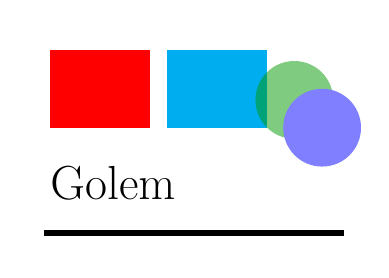
\begin{tikzpicture}[x=1bp,y=-1bp,inner sep=0pt]
  \useasboundingbox (0,0) rectangle (120,80);
  \fill[white] (0,0) rectangle (120,80);
  \draw[black,line width=2bp] (6,74) -- (114,74);
  \definecolor{red}{RGB}{255,0,0}
  \definecolor{cyan}{cmyk}{1,0,0,0}
  \fill[red] (8,8) rectangle (44,36);
  \fill[cyan] (50,8) rectangle (86,36);
  \begin{scope}[transparency group,opacity=0.5]
    \fill[green!60!black] (96,26) circle (14);
    \fill[blue] (106,36) circle (14);
  \end{scope}
  \node[anchor=base west,font=\fontsize{16bp}{16bp}\selectfont] at (8,62) {Golem};
\end{tikzpicture}
\end{document}
